
The workflow is depicted in Figure \ref{fig:protocol}, and described with full details as follows.

\begin{figure}[h]
	\centering
		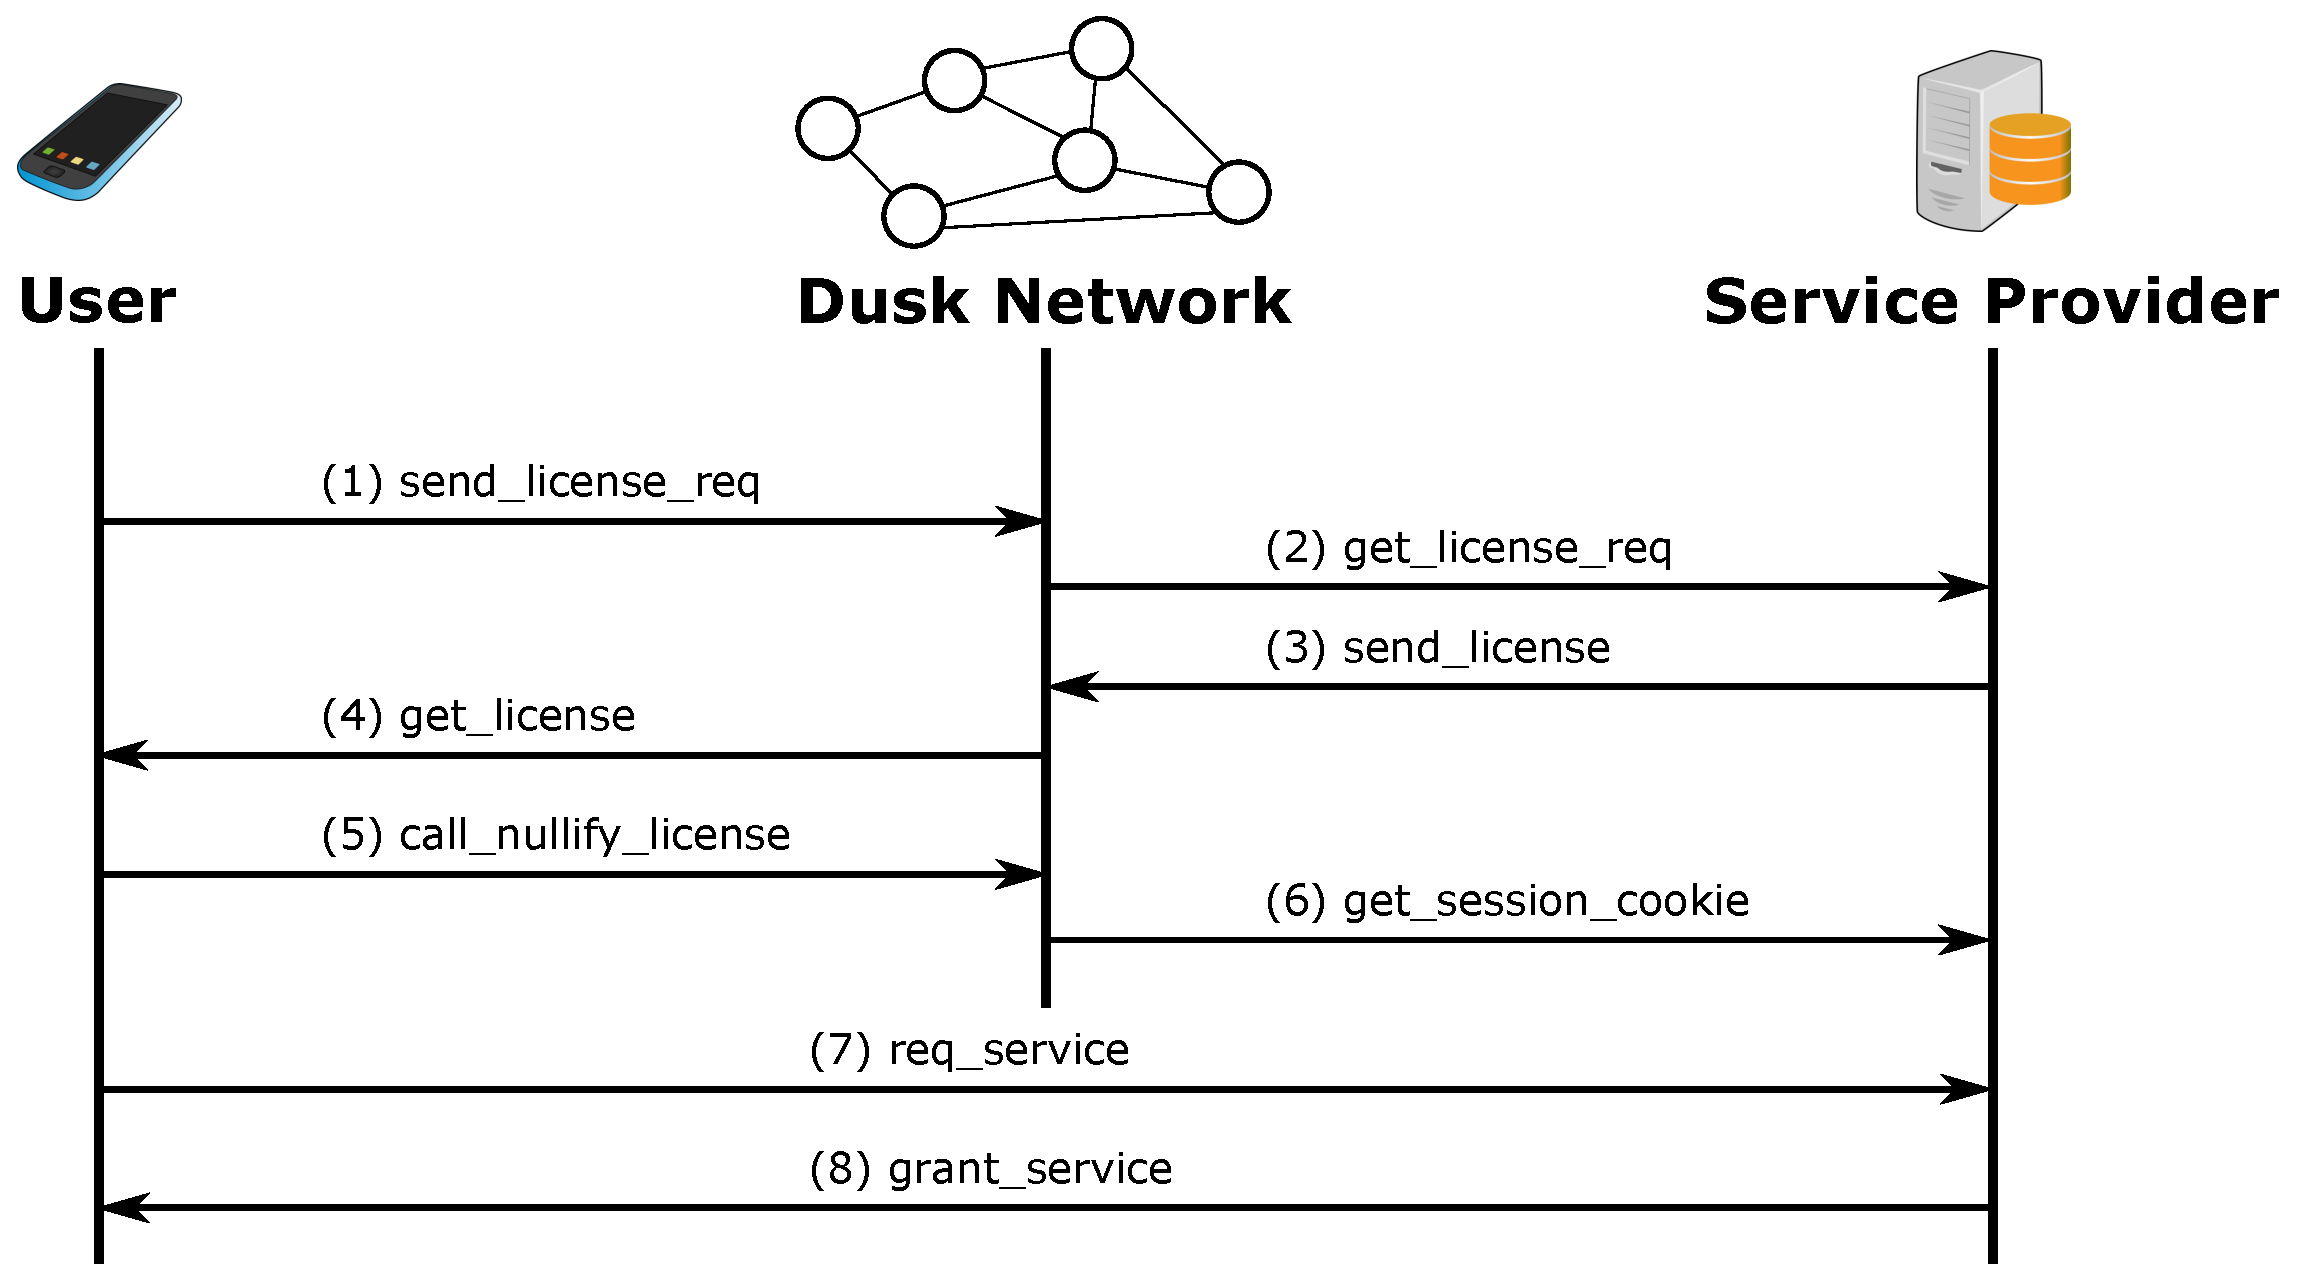
\includegraphics[width=390pt,draft=false]{images/protocol.eps}
	\caption{Overview of the protocol messages exchanged between the user, the Dusk Network, and the SP.}
	\label{fig:protocol}
\end{figure}

\begin{enumerate}
	\item (\textbf{user}) $\mathsf{send\_note\_license\_req}$ : Compute a note public key $(\npk_{\user}, R_{\user})$ belonging to the user, using the user's own public key, and also an additional key $\ksym_{\user} = \hp(\npk_{\user}, \nsk_{\user})$, by computing first the user's $\nsk_{\user}$. Then, send the required amount of Dusk coins to the SP, in order to pay for the service. Into the same transaction, send an NFT to the SP using the function $\mintnft(\npk_{\SP}, R_{\SP}, \nftpayload, \kdh)$, whose arguments are computed as follows:
	\begin{itemize}
		\item $(\npk_{\SP}, R_{\SP})$ is the SP's note public key, computed through his public key $\pk_{\SP}$.
		\item $\nftpayload = (\npk_{\user}, R_{\user}, \ksym_{\user})$.
		\item $\kdh$ is computed using the SP's public key.
	\end{itemize}

	\item (\textbf{SP}) $\mathsf{get\_note\_license\_req}$ : Continuously check the network for incoming license requests. Upon receiving the payment from a user, define a set of attributes $attr$ representing the license, and compute a digital signature as follows:

	$$\lsig= \sign_{\sk_{\SP}}(\npk_{\user}, \attr)$$

	\item (\textbf{SP}) $\mathsf{send\_note\_license}$ : Set the $\nftpayload = \{\lsig, \attr\}$, and send the license to the user using the function $\mintnft(\npk_{\user}, R_{\user}, \nftpayload, \ksym_{\user})$.

	\item (\textbf{user}) $\mathsf{get\_note\_license}$ : Receive the note containing the license. 

	\item (\textbf{user}) $\mathsf{call\_nullify\_license}$ : When desiring to use the license, nullify it by executing a call to the license contract. The following steps are performed:

	\begin{itemize}
		\item The user sets a session cookie $\stoken = (\mathsf{s_0}, \mathsf{s_1}, \mathsf{s_2}) \leftarrow \F_t$.
		\item The user creates a new NFT note where $\nftpayload = \stoken$, and the SP is the receiver.
		\item The user issues the transaction that includes the NFT described in the previous step, by calling the license contract. In this case, the \textsf{tx\_proof} is computed as done in the standard Phoenix model, but into the same circuit, the circuit depicted in Figure \ref{fig:circuit_prove_nft} is appended.
		\item The network validators will execute the smart contract, which verifies the proof. Upon success, the NFT note will be forwarded, and the license nullifier $\lnullifier$ will be added to the Merkle tree of nullifiers.
	\end{itemize}

	\item (\textbf{SP}) $\mathsf{get\_note\_session\_cookie}$ : Receive a note containing the session cookie $\stoken$.

	\item (\textbf{user}) $\mathsf{req\_service}$ : Request the service to the SP, establishing communication using a secure channel, and providing the tuple $(\mathsf{tx\_hash}, \pk_{\SP}, \attr, c, \stoken)$.

	\item (\textbf{SP}) $\mathsf{grant\_service}$ : Grant or deny the service upon verification of the following steps:

	\begin{itemize}
		\item Check whether or not the values $(\attr, \pk_{\SP}, c)$ are correct.
		\item Check whether or not the openings $((\pk_{\SP}, \mathsf{s_0}), (\attr, \mathsf{s_1}), (c, \mathsf{s_2}))$ match the commitments $\com_0^{hash}, \com_1, \com_2$ found in the transaction $\mathsf{tx\_hash}$.
	\end{itemize}

\end{enumerate}

\begin{figure}[h]
	\centering
	\setlength{\fboxsep}{5pt}%
	\setlength{\fboxrule}{0.3pt}%
	\fbox{
		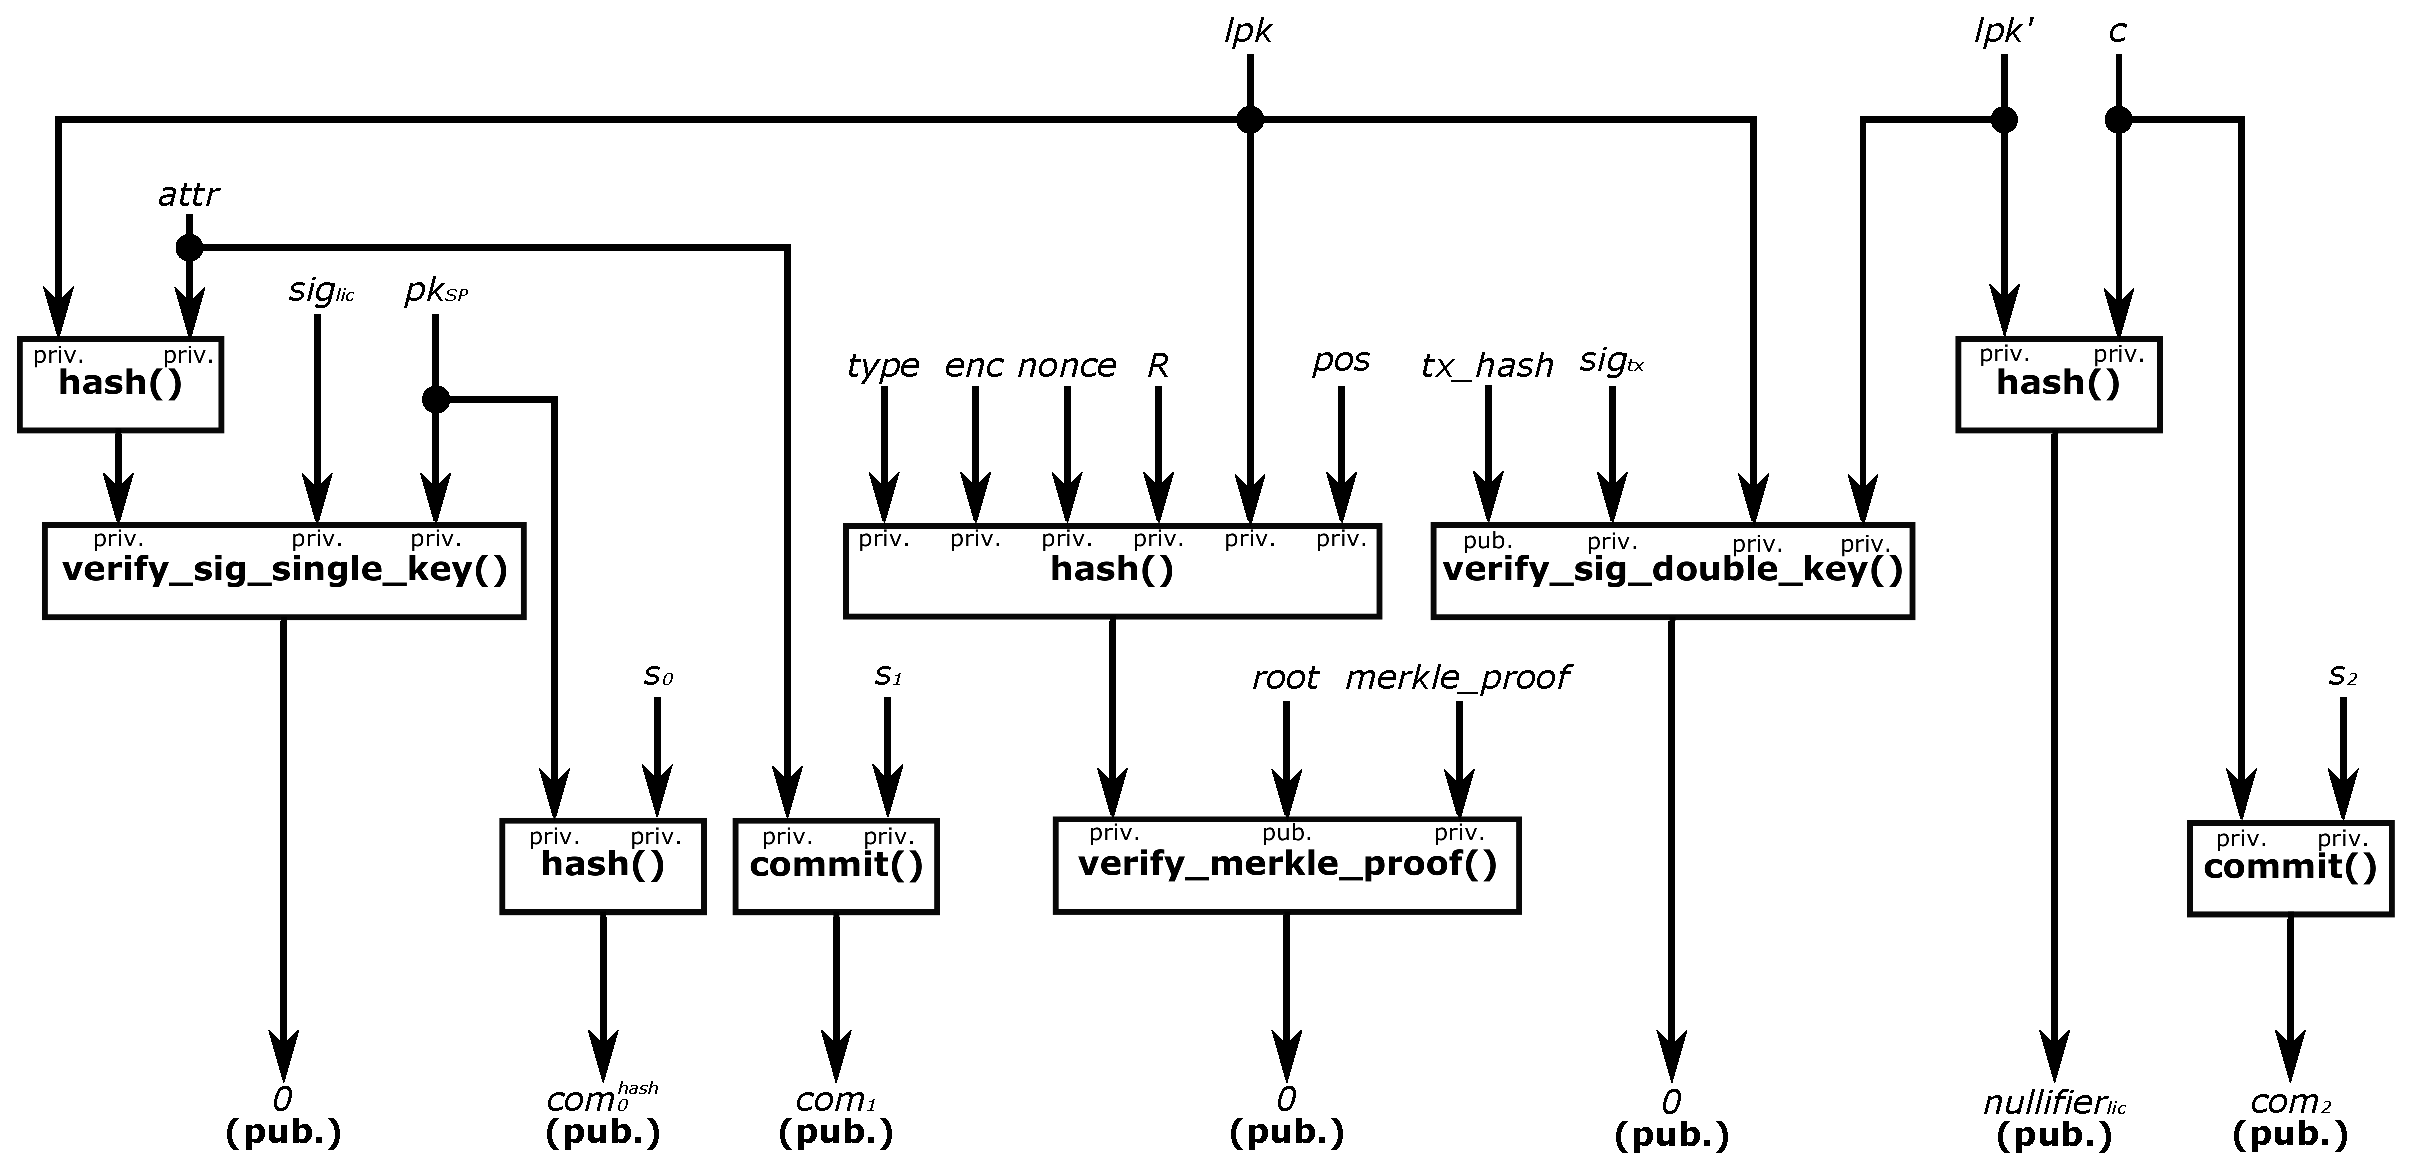
\includegraphics[width=460pt,draft=false]{images/circuit_prove_nft.eps}}
	\caption{Arithmetic circuit for proving a license's ownership.}
	\label{fig:circuit_prove_nft}
\end{figure}

Furthermore, the SP might request the user to nullify the license they are using (i.e. this is a single-use license, like entering a concert). This is done through the computation of $\lnullifier$. The deployment of this part of the circuit has two different possibilities:
\begin{itemize}
	\item If we set $c = 0$ (or directly remove this input from the circuit), the license will be able to be used only once.
	\item If the SP requests the user to set a custom value for $c$ (e.g. the date of an event), the license will be able to be reused only under certain conditions.
\end{itemize}
